\documentclass[10pt]{article}

\input{/Users/gabesekeres/Dropbox/LaTeX_Docs/pset_preamble.tex}

\course{ECON 6140}
\pset{6}
\begin{document}
\maketitle

\begin{enumerate}
	\item The household solves the Lagrangian\[\mathcal{L} = \expect_0 \sum_{t=0}^\infty \beta^t \barl U(C_t,N_t) + \lambda_t \parl B_{t-1} + W_tN_t + D_t - P_tC_t- Q_tB_t\parr\barr\]which admits the first order conditions\begin{align*} \frac{\partial \mathcal{L}}{\partial C_t} &: \beta^t(U_{c,t} - \lambda_t P_t)=0 \\ \frac{\partial \mathcal{L}}{\partial N_t} &: \beta^t (U_{n,t} - \lambda_t W_t) = 0 \\ \frac{\partial \mathcal{L}}{\partial B_t} &: \beta^{t+1} \expect_t \lambda_{t+1} - \beta^t \lambda_t Q_t = 0\end{align*}Since we have that $U(C_t,N_t) = \frac{C_t^{1-\sigma}-1}{1-\sigma} - \frac{N_t^{1+\varphi}}{1+\varphi}$, the household's optimality conditions become\begin{align*} \frac{N_t^{\varphi}}{C_t^{-\sigma}} &= \frac{W_t}{P_t} \\ C_t^{-\sigma} &= \beta Q_t^{-1} \expect_t \barl C_{t+1}^{-\sigma} \frac{P_t}{P_{t+1}}\barr\end{align*}The firm's optimality condition with the standard production function is, as always,\[\frac{W_t}{P_t} = (1-\alpha)A_t N_t^{-\alpha}\]We will log-linearize these conditions, and using the typical lowercase variables, get the optimality conditions:\begin{align*} \varphi n_t + \sigma c_t &= w_t - p_t \\ c_t &= \expect_t[c_{t+1}] - \frac{1}{\sigma} \parl i_t - \rho - \expect_t[\pi_{t+1}]\parr \\ w_t - p_t &= \ln(1-\alpha) + a_t - \alpha n_t\end{align*}Along with the market clearing condition ($y_t = c_t$), this allows us to solve for explicit forms for the the endogenous variables (omitting the arithmetic because it's in the section notes): \begin{align*} n_t &= \frac{(1-\sigma)a_t + \ln(1-\alpha)}{\varphi + \alpha + \sigma(1-\alpha)} = \psi_{na} a_t + \psi_n \\ y_t &= a_t + (1-\alpha)n_t = \psi_{ya} a_t + \psi_y \\ \omega_t &= \ln(1-\alpha) + a_t -\alpha n_t = \psi_{\omega a}a_t + \psi_\omega\end{align*}where the $\psi$ variables are as we defined in class; see Table~\ref{tab:vars} \begin{table}[H]\label{tab:vars}\centering \begin{tabular}{c|c|c|c|c|c} $\psi$ & Expression & (1) Value & (4) Value & (5) Value & (6) Value \\\hline $\psi_{na}$ & $\frac{1-\sigma}{\varphi + \alpha + \sigma(1-\alpha)}$ & $-0.2128$ & $0.137$ & $-0.0855$ & $-0.2222$ \\\hline $\psi_n$ & $\frac{\ln(1-\alpha)}{\varphi + \alpha + \sigma(1-\alpha)}$ & $-0.0759$ & $-0.0977$ & $-0.0305$ & $-0.1540$ \\\hline $\psi_{ya}$ & $\frac{1+\varphi}{\varphi + \alpha + \sigma(1-\alpha)}$ & $0.8511$ & $1.0959$ & $0.9402$ & $0.8889$ \\\hline $\psi_y$ & $\frac{(1-\alpha)\ln(1-\alpha)}{\varphi + \alpha + \sigma(1-\alpha)}$ & $-0.0531$ & $-0.0684$ & $-0.0213$ & $-0.0770$ \\\hline $\psi_{\omega a}$ & $\frac{\varphi +\sigma}{\varphi + \alpha + \sigma(1-\alpha)}$ & $1.0638$ & $0.9589$ & $1.0256$ & $1.1111$ \\\hline $\psi_\omega$ & $\frac{(\varphi + \sigma (1-\alpha))\ln(1-\alpha)}{\varphi + \alpha + \sigma(1-\alpha)}$ & $-0.3339$ & $-0.3274$ & $-0.3475$ & $-0.6161$\end{tabular}\caption{Model Parameterizations (values approximate)}\end{table}
	\item \textbf{\textit{n.b.}} All code is below in the \href{code}{code section} \\\\ I simulated 100 periods of $a_t$, using seed 1234 in Julia for replicability. The plotted time series values are Figure~\ref{fig:q2sim} \begin{figure}[H] \centering 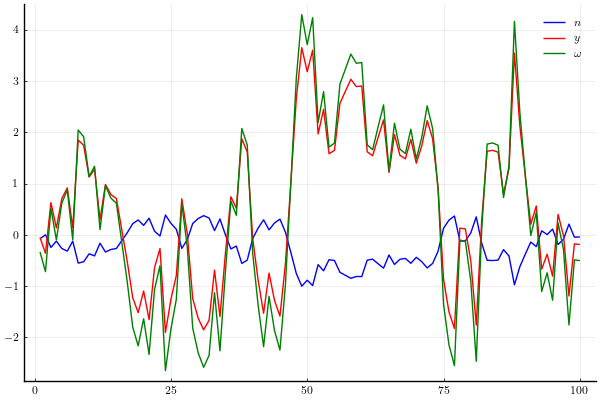
\includegraphics[width=12cm]{q2_simdata.png}\caption{Simulated Economy Under Initial Parameters} \label{fig:q2sim}\end{figure} The sample variances are\[\parl \var(n),\var(y),\var(\omega)\parr = (0.1322, 2.1154, 3.3054)\]and the sample cross-variable correlations are\[\matrixc{\corr(n,n) & \corr(n,y) & \corr(n,\omega) \\ \corr(y,n) & \corr(y,y) & \corr(y,\omega) \\ \corr(\omega,n) & \corr(\omega,y) & \corr(n,\omega)} = \matrixc{1.0 &-1.0 &-1.0\\ -1.0& 1.0 &1.0\\ -1.0& 1.0& 1.0}\]These sample moments are exactly correlated, where even under restrictive assumptions we would not expect the population moments to all be precisely 1. This happens because we assume linearity, and so all of the time series are linear transformations of each other, so they are perfectly correlated.
	\item I computed the impulse response functions over 20 periods, and plotted them in Figure~\ref{fig:q2irf} \begin{figure}[H] \centering 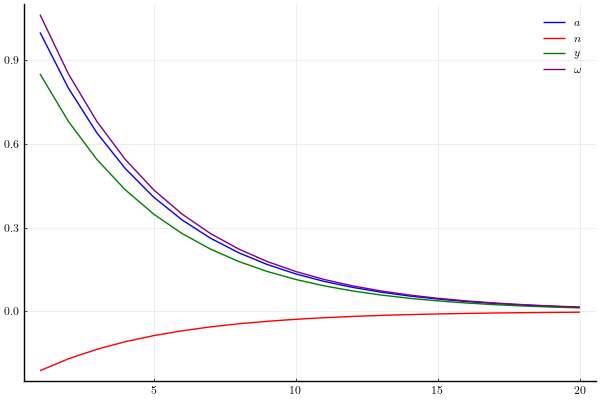
\includegraphics[width=12cm]{q2_irf.png} \caption{Impulse Response Functions Under Initial Parameters} \label{fig:q2irf}\end{figure}
	\item I set $\sigma = 0.5$, and ran the same code as in questions (2) and (3). The simulated economy is plotted in Figure~\ref{fig:q4sim} \begin{figure}[H] \centering 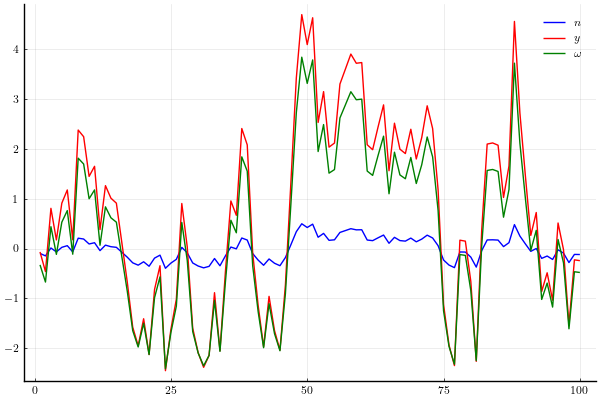
\includegraphics[width=12cm]{q4_simdata.png}\caption{Simulated Economy When $\sigma = 0.5$} \label{fig:q4sim}\end{figure} The sample variances are\[\parl \var(n),\var(y),\var(\omega)\parr = (0.0548, 3.5076, 2.6855)\]and the sample cross-variable correlations are\[\matrixc{\corr(n,n) & \corr(n,y) & \corr(n,\omega) \\ \corr(y,n) & \corr(y,y) & \corr(y,\omega) \\ \corr(\omega,n) & \corr(\omega,y) & \corr(n,\omega)} = \matrixc{1.0 &1.0 &1.0\\ 1.0& 1.0 &1.0\\ 1.0& 1.0& 1.0}\]Note that now everything is exactly correlated positively! In other words, as the coefficient of relative risk aversion decreases, the household will actually increase their work when their productivity increases, rather than otherwise. The impulse response functions are plotted in Figure~\ref{fig:q4irf} \begin{figure}[H] \centering 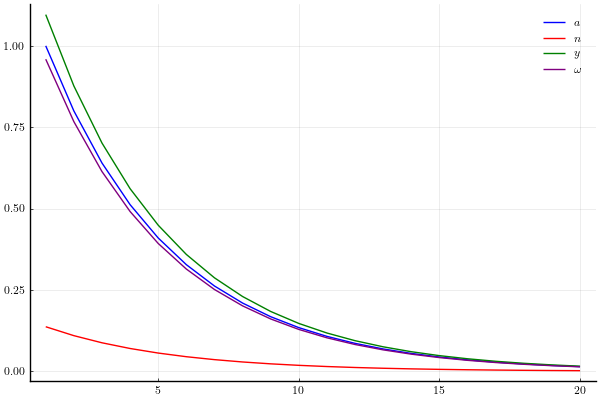
\includegraphics[width=12cm]{q4_irf.png} \caption{Impulse Response Functions When $\sigma = 0.5$} \label{fig:q4irf}\end{figure}Note that the variables now move in the same direction.
	\item I set $\varphi=10$, and ran the same code as in questions (2) and (3). The simulated economy is plotted in Figure~\ref{fig:q5sim} \begin{figure}[H] \centering 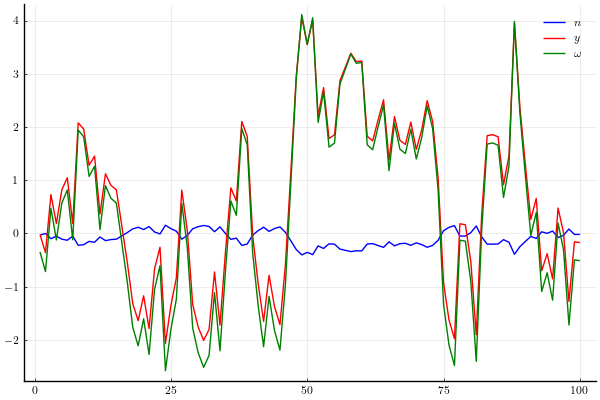
\includegraphics[width=12cm]{q5_simdata.png}\caption{Simulated Economy When $\varphi=10$} \label{fig:q5sim}\end{figure} The sample variances are\[\parl \var(n),\var(y),\var(\omega)\parr = (0.0213, 2.5816, 3.0723)\]and the sample cross-variable correlations are\[\matrixc{\corr(n,n) & \corr(n,y) & \corr(n,\omega) \\ \corr(y,n) & \corr(y,y) & \corr(y,\omega) \\ \corr(\omega,n) & \corr(\omega,y) & \corr(n,\omega)} = \matrixc{1.0 &-1.0 &-1.0\\ -1.0& 1.0 &1.0\\- 1.0& 1.0& 1.0}\] The impulse response functions are plotted in Figure~\ref{fig:q5irf} \begin{figure}[H] \centering 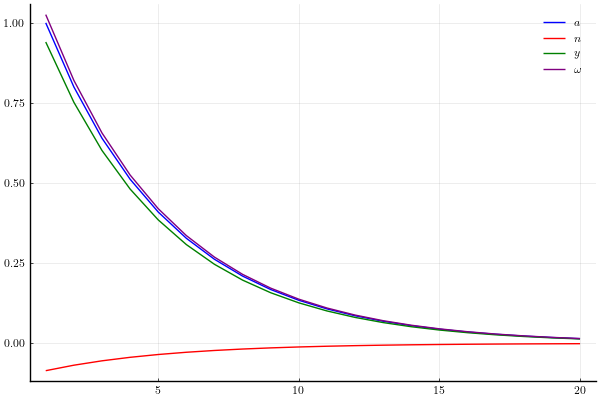
\includegraphics[width=10cm]{q5_irf.png} \caption{Impulse Response Functions When $\varphi = 10$} \label{fig:q5irf}\end{figure}Note that now $a$, $y$, and $\omega$ are extremely closely correlated, even more than in part (2). The interpretation here is that as leisure becomes more valuable, the household works even less, getting closer to the minimum.
	\item I set $\alpha=0.5$, and ran the same code as in questions (2) and (3). The simulated economy is plotted in Figure~\ref{fig:q6sim} \begin{figure}[H] \centering 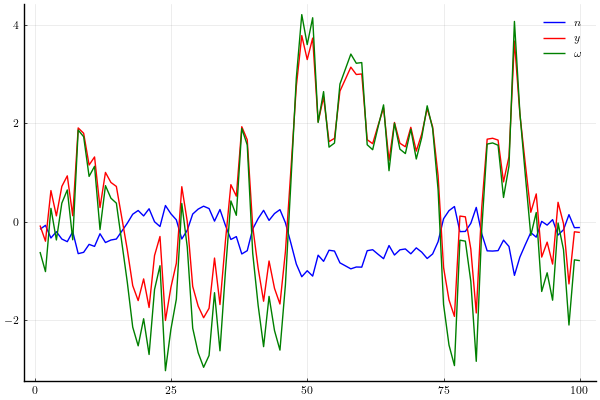
\includegraphics[width=12cm]{q6_simdata.png}\caption{Simulated Economy When $\alpha=0.5$} \label{fig:q6sim}\end{figure} The sample variances are\[\parl \var(n),\var(y),\var(\omega)\parr = (0.1442, 2.3077, 3.6057)\]and the sample cross-variable correlations are\[\matrixc{\corr(n,n) & \corr(n,y) & \corr(n,\omega) \\ \corr(y,n) & \corr(y,y) & \corr(y,\omega) \\ \corr(\omega,n) & \corr(\omega,y) & \corr(n,\omega)} = \matrixc{1.0 &-1.0 &-1.0\\ -1.0& 1.0 &1.0\\- 1.0& 1.0& 1.0}\] The impulse response functions are plotted in Figure~\ref{fig:q6irf} \begin{figure}[H] \centering 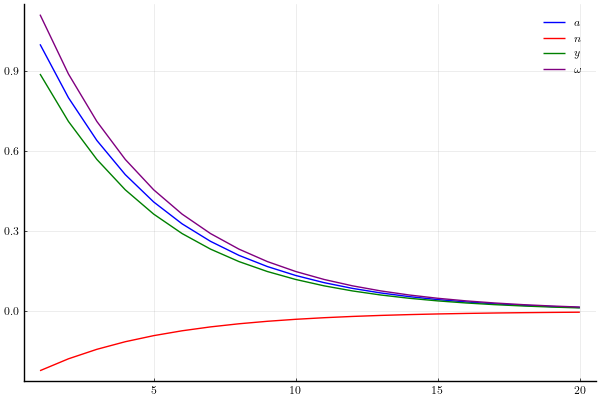
\includegraphics[width=10cm]{q6_irf.png} \caption{Impulse Response Functions When $\alpha=0.5$} \label{fig:q6irf}\end{figure}This is the closest to the initial case, and the interpretation here is that as $\alpha$ increases, workers will care more about current period consumption and less about leisure, as can be seen from their first order conditions.
	\item In the main model, the standard deviation of the output gap is $\text{std }y_t = 1.4545$, as opposed to the typical standard deviation of 2. If we wanted the standard deviation in this model to match the data, we would change $\psi_{ya}$, so that a change in $a_t$ would differently change $y_t$. Specifically, I found that the most straightforward change was to move $\sigma$ to $\frac{1}{3}$, which led to a standard deviation of $1.936$.
\end{enumerate}



\newpage
\section*{Code}\label{code}

I defined the relevant functions in a file called \texttt{functions.jl}, which is:

\lstinputlisting[language=Julia]{functions.jl}

\newpage
I ran the rest of the code from a file called \texttt{main.jl}, which is:

\lstinputlisting[language=Julia]{main.jl}







\end{document}